%% uncomment to list all files in log
%\listfiles

\documentclass[12pt]{report}


\usepackage{fontspec}

%\setmainfont[Scale=MatchLowercase]{Lucida Bright}
%\setmonofont{FreeMono}
%\setmonofont{Source Code Pro}
\setmonofont[Scale=MatchLowercase]{Ubuntu Mono}

\usepackage[headings]{fullpage}

% national use characters 
%\usepackage{inputenc}

% ams mathematical symbols
\usepackage{amsmath,amssymb}

% added to support pandoc highlighting
\usepackage{microtype}

\usepackage{makeidx}

% add index and bibliographies to table of contents
\usepackage[nottoc]{tocbibind}

% postscript courier and times in place of cm fonts
%\usepackage{courier}
%\usepackage{times}

% extended coloring
\usepackage{color}
\usepackage[table,dvipsnames]{xcolor}
\usepackage{colortbl}

% advanced date formating
\usepackage{datetime}

%support pandoc code highlighting
\usepackage{fancyvrb}
\DefineShortVerb[commandchars=\\\{\}]{\|}
\DefineVerbatimEnvironment{Highlighting}{Verbatim}{commandchars=\\\{\}}
% Add ',fontsize=\small' for more characters per line

%tango style colors
% \usepackage{framed}
% \definecolor{shadecolor}{RGB}{255,255,255}
% \newenvironment{Shaded}{\begin{snugshade}}{\end{snugshade}}
% \newcommand{\KeywordTok}[1]{\textcolor[rgb]{0.13,0.29,0.53}{\textbf{{#1}}}}
% \newcommand{\DataTypeTok}[1]{\textcolor[rgb]{0.13,0.29,0.53}{{#1}}}
% \newcommand{\DecValTok}[1]{\textcolor[rgb]{0.00,0.00,0.81}{{#1}}}
% \newcommand{\BaseNTok}[1]{\textcolor[rgb]{0.00,0.00,0.81}{{#1}}}
% \newcommand{\FloatTok}[1]{\textcolor[rgb]{0.00,0.00,0.81}{{#1}}}
% \newcommand{\CharTok}[1]{\textcolor[rgb]{0.31,0.60,0.02}{{#1}}}
% \newcommand{\StringTok}[1]{\textcolor[rgb]{0.31,0.60,0.02}{{#1}}}
% \newcommand{\CommentTok}[1]{\textcolor[rgb]{0.56,0.35,0.01}{\textit{{#1}}}}
% \newcommand{\OtherTok}[1]{\textcolor[rgb]{0.56,0.35,0.01}{{#1}}}
% \newcommand{\AlertTok}[1]{\textcolor[rgb]{0.94,0.16,0.16}{{#1}}}
% \newcommand{\FunctionTok}[1]{\textcolor[rgb]{0.00,0.00,0.00}{{#1}}}
% \newcommand{\RegionMarkerTok}[1]{{#1}}
% \newcommand{\ErrorTok}[1]{\textbf{{#1}}}
% \newcommand{\NormalTok}[1]{{#1}}

%espresso style colors
% \usepackage{framed}
% \definecolor{shadecolor}{RGB}{42,33,28}
% \newenvironment{Shaded}{\begin{snugshade}}{\end{snugshade}}
% \newcommand{\KeywordTok}[1]{\textcolor[rgb]{0.26,0.66,0.93}{\textbf{{#1}}}}
% \newcommand{\DataTypeTok}[1]{\textcolor[rgb]{0.74,0.68,0.62}{\underline{{#1}}}}
% \newcommand{\DecValTok}[1]{\textcolor[rgb]{0.27,0.67,0.26}{{#1}}}
% \newcommand{\BaseNTok}[1]{\textcolor[rgb]{0.27,0.67,0.26}{{#1}}}
% \newcommand{\FloatTok}[1]{\textcolor[rgb]{0.27,0.67,0.26}{{#1}}}
% \newcommand{\CharTok}[1]{\textcolor[rgb]{0.02,0.61,0.04}{{#1}}}
% \newcommand{\StringTok}[1]{\textcolor[rgb]{0.02,0.61,0.04}{{#1}}}
% \newcommand{\CommentTok}[1]{\textcolor[rgb]{0.00,0.40,1.00}{\textit{{#1}}}}
% \newcommand{\OtherTok}[1]{\textcolor[rgb]{0.74,0.68,0.62}{{#1}}}
% \newcommand{\AlertTok}[1]{\textcolor[rgb]{1.00,1.00,0.00}{{#1}}}
% \newcommand{\FunctionTok}[1]{\textcolor[rgb]{1.00,0.58,0.35}{\textbf{{#1}}}}
% \newcommand{\RegionMarkerTok}[1]{\textcolor[rgb]{0.74,0.68,0.62}{{#1}}}
% \newcommand{\ErrorTok}[1]{\textcolor[rgb]{0.74,0.68,0.62}{\textbf{{#1}}}}
% \newcommand{\NormalTok}[1]{\textcolor[rgb]{0.74,0.68,0.62}{{#1}}}

%kete style colors
% \newenvironment{Shaded}{}{}
% \newcommand{\KeywordTok}[1]{\textbf{{#1}}}
% \newcommand{\DataTypeTok}[1]{\textcolor[rgb]{0.50,0.00,0.00}{{#1}}}
% \newcommand{\DecValTok}[1]{\textcolor[rgb]{0.00,0.00,1.00}{{#1}}}
% \newcommand{\BaseNTok}[1]{\textcolor[rgb]{0.00,0.00,1.00}{{#1}}}
% \newcommand{\FloatTok}[1]{\textcolor[rgb]{0.50,0.00,0.50}{{#1}}}
% \newcommand{\CharTok}[1]{\textcolor[rgb]{1.00,0.00,1.00}{{#1}}}
% \newcommand{\StringTok}[1]{\textcolor[rgb]{0.87,0.00,0.00}{{#1}}}
% \newcommand{\CommentTok}[1]{\textcolor[rgb]{0.50,0.50,0.50}{\textit{{#1}}}}
% \newcommand{\OtherTok}[1]{{#1}}
% \newcommand{\AlertTok}[1]{\textcolor[rgb]{0.00,1.00,0.00}{\textbf{{#1}}}}
% \newcommand{\FunctionTok}[1]{\textcolor[rgb]{0.00,0.00,0.50}{{#1}}}
% \newcommand{\RegionMarkerTok}[1]{{#1}}
% \newcommand{\ErrorTok}[1]{\textcolor[rgb]{1.00,0.00,0.00}{\textbf{{#1}}}}
% \newcommand{\NormalTok}[1]{{#1}}
%end pandoc code hacks

% jodliterate colors
\usepackage{color}
\definecolor{shadecolor}{RGB}{248,248,248}
% j control structures 
\definecolor{keywcolor}{rgb}{0.13,0.29,0.53}
% j explicit arguments x y m n u v
\definecolor{datacolor}{rgb}{0.13,0.29,0.53}
% j numbers - all types see j.xml
\definecolor{decvcolor}{rgb}{0.00,0.00,0.81}
\definecolor{basencolor}{rgb}{0.00,0.00,0.81}
\definecolor{floatcolor}{rgb}{0.00,0.00,0.81}
% j local assignments
\definecolor{charcolor}{rgb}{0.31,0.60,0.02}
\definecolor{stringcolor}{rgb}{0.31,0.60,0.02}
\definecolor{commentcolor}{rgb}{0.56,0.35,0.01}
% primitive adverbs and conjunctions
%\definecolor{othercolor}{rgb}{0.56,0.35,0.01}   
\definecolor{othercolor}{RGB}{0,0,255}
% global assignments
\definecolor{alertcolor}{rgb}{0.94,0.16,0.16}
% primitive J verbs and noun names
\definecolor{funccolor}{rgb}{0.00,0.00,0.00}    

\usepackage{framed}
\newenvironment{Shaded}{}{}
\newcommand{\KeywordTok}[1]{\textcolor{keywcolor}{\textbf{{#1}}}}
\newcommand{\DataTypeTok}[1]{\textcolor{datacolor}{{#1}}}
%\newcommand{\DecValTok}[1]{\textcolor{decvcolor}{{#1}}}
\newcommand{\DecValTok}[1]{{#1}} 
\newcommand{\BaseNTok}[1]{\textcolor{basencolor}{{#1}}}
\newcommand{\FloatTok}[1]{\textcolor{floatcolor}{{#1}}}
\newcommand{\CharTok}[1]{\textcolor{charcolor}{\textbf{{#1}}}}
\newcommand{\StringTok}[1]{\textcolor{stringcolor}{{#1}}}
\newcommand{\CommentTok}[1]{\textcolor{commentcolor}{\textit{{#1}}}}
\newcommand{\OtherTok}[1]{\textcolor{othercolor}{{#1}}} 
\newcommand{\AlertTok}[1]{\textcolor{alertcolor}{\textbf{{#1}}}}
%\newcommand{\FunctionTok}[1]{\textcolor{funccolor}{{#1}}}
\newcommand{\FunctionTok}[1]{{#1}}
\newcommand{\RegionMarkerTok}[1]{{#1}}
\newcommand{\ErrorTok}[1]{\textbf{{#1}}}
\newcommand{\NormalTok}[1]{{#1}}

% headers and footers
\usepackage{fancyhdr}
\pagestyle{fancy}

\fancyhead{}
\fancyfoot{}

%\fancyhead[LE,RO]{\slshape \rightmark}
%\fancyhead[LO,RE]{\slshape \leftmark}
\fancyfoot[C]{\thepage}
%\headrulewidth 0.4pt
%\footrulewidth 0 pt

%\addtolength{\headheight}{\baselineskip}

%\lfoot{\emph{Analyze the Data not the Drivel}}
%\rfoot{\emph{\today}}

% subfigure handles figures that contain subfigures
%\usepackage{color,graphicx,subfigure,sidecap}
\usepackage{graphicx,sidecap}
\usepackage{subfigure}
\graphicspath{{./inclusions/}}

% floatflt provides for text wrapping around small figures and tables
\usepackage{floatflt}

% tweak caption formats 
\usepackage{caption} 
\usepackage{sidecap}
%\usepackage{subcaption} % not compatible with subfigure

\usepackage{rotating} % flip tables sideways

% complex footnotes
%\usepackage{bigfoot}

% weird logos \XeLaTeX
\usepackage{metalogo}

% source code listings
\usepackage{listings}

% long tables
% \usepackage{longtable}

\newcommand{\HRule}{\rule{\linewidth}{0.5mm}}

% map LaTeX cross references into PDF cross references
\usepackage[
            %dvips,
            colorlinks,
            linkcolor=blue,
            citecolor=blue,
            urlcolor=blue,   % magenta, cyan default        
            pdfauthor={John D. Baker},
            pdftitle={Analyze the Data not the Drivel},
            pdfsubject={Blog},
            pdfcreator={MikTeX+LaTeXe with hyperref package},
            pdfkeywords={blog,wordpress},
            ]{hyperref}
           
% custom colors
\definecolor{CodeBackGround}{cmyk}{0.0,0.0,0,0.05}    % light gray
\definecolor{CodeComment}{rgb}{0,0.50,0.00}           % dark green {0,0.45,0.08}
\definecolor{TableStripes}{gray}{0.9}                 % odd/even background in tables

\lstdefinelanguage{bat}
{morekeywords={echo,title,pushd,popd,setlocal,endlocal,off,if,not,exist,set,goto,pause},
sensitive=True,
morecomment=[l]{rem}
}

\lstdefinelanguage{jdoc}
{
morekeywords={},
otherkeywords={assert.,break.,continue.,for.,do.,if.,else.,elseif.,return.,select.,end.
,while.,whilst.,throw.,catch.,catchd.,catcht.,try.,case.,fcase.},
sensitive=True,
morecomment=[l]{NB.},
morestring=[b]',
morestring=[d]',
}

% latex size ordering - can never remember it
% \tiny
% \scriptsize
% \footnotesize
% \small
% \normalsize
% \large
% \Large
% \LARGE
% \huge
% \Huge
 
% listings package settings  
\lstset{%
  language=jdoc,                                % j document settings
  basicstyle=\ttfamily\footnotesize,            
  keywordstyle=\bfseries\color{keywcolor}\footnotesize,
  identifierstyle=\color{black},
  commentstyle=\slshape\color{CodeComment},     % colored slanted comments
  stringstyle=\color{red}\ttfamily,
  showstringspaces=false,                       
  %backgroundcolor=\color{CodeBackGround},       
  frame=single,                                
  framesep=1pt,                                 
  framerule=0.8pt,                             
  rulecolor=\color{CodeBackGround},   
  showspaces=false,
  %columns=fullflexible,
  %numbers=left,
  %numberstyle=\footnotesize,
  %numbersep=9pt,
  tabsize=2,
  showtabs=false,
  captionpos=b
  breaklines=true,                              
  breakindent=5pt                              
}

\lstdefinelanguage{JavaScript}{
  keywords={typeof, new, true, false, catch, function, return, null, catch, switch, var, if, in, while, do, else, case, break},
  ndkeywords={class, export, boolean, throw, implements, import, this},
  ndkeywordstyle=\color{darkgray}\bfseries,
  sensitive=false,
  comment=[l]{//},
  morecomment=[s]{/*}{*/},
  morestring=[b]',
  morestring=[b]"
}

% C# settings
\lstdefinestyle{sharpc}{
language=[Sharp]C,
basicstyle=\ttfamily\scriptsize, 
keywordstyle=\bfseries\color{keywcolor}\scriptsize,
framerule=0pt
}

% for source code listing longer than two use smaller font
\lstdefinestyle{smallersource}{
basicstyle=\ttfamily\scriptsize, 
keywordstyle=\bfseries\color{keywcolor}\scriptsize,
framerule=0pt
}

\lstdefinestyle{resetdefaults}{
language=jdoc,
basicstyle=\ttfamily\footnotesize,  
keywordstyle=\bfseries\color{keywcolor}\footnotesize,                                                               
framerule=0.8pt 
}

% APL UTF8 code points listed for lstlisting processing
\makeatletter
\lst@InputCatcodes
\def\lst@DefEC{%
 \lst@CCECUse \lst@ProcessLetter
  ^^80^^81^^82^^83^^84^^85^^86^^87^^88^^89^^8a^^8b^^8c^^8d^^8e^^8f%
  ^^90^^91^^92^^93^^94^^95^^96^^97^^98^^99^^9a^^9b^^9c^^9d^^9e^^9f%
  ^^a0^^a1^^a2^^a3^^a4^^a5^^a6^^a7^^a8^^a9^^aa^^ab^^ac^^ad^^ae^^af%
  ^^b0^^b1^^b2^^b3^^b4^^b5^^b6^^b7^^b8^^b9^^ba^^bb^^bc^^bd^^be^^bf%
  ^^c0^^c1^^c2^^c3^^c4^^c5^^c6^^c7^^c8^^c9^^ca^^cb^^cc^^cd^^ce^^cf%
  ^^d0^^d1^^d2^^d3^^d4^^d5^^d6^^d7^^d8^^d9^^da^^db^^dc^^dd^^de^^df%
  ^^e0^^e1^^e2^^e3^^e4^^e5^^e6^^e7^^e8^^e9^^ea^^eb^^ec^^ed^^ee^^ef%
  ^^f0^^f1^^f2^^f3^^f4^^f5^^f6^^f7^^f8^^f9^^fa^^fb^^fc^^fd^^fe^^ff%
  ^^^^20ac^^^^0153^^^^0152%
  ^^^^20a7^^^^2190^^^^2191^^^^2192^^^^2193^^^^2206^^^^2207^^^^220a%
  ^^^^2218^^^^2228^^^^2229^^^^222a^^^^2235^^^^223c^^^^2260^^^^2261%
  ^^^^2262^^^^2264^^^^2265^^^^2282^^^^2283^^^^2296^^^^22a2^^^^22a3%
  ^^^^22a4^^^^22a5^^^^22c4^^^^2308^^^^230a^^^^2336^^^^2337^^^^2339%
  ^^^^233b^^^^233d^^^^233f^^^^2340^^^^2342^^^^2347^^^^2348^^^^2349%
  ^^^^234b^^^^234e^^^^2350^^^^2352^^^^2355^^^^2357^^^^2359^^^^235d%
  ^^^^235e^^^^235f^^^^2361^^^^2362^^^^2363^^^^2364^^^^2365^^^^2368%
  ^^^^236a^^^^236b^^^^236c^^^^2371^^^^2372^^^^2373^^^^2374^^^^2375%
  ^^^^2377^^^^2378^^^^237a^^^^2395^^^^25af^^^^25ca^^^^25cb%  
  ^^00}
\lst@RestoreCatcodes
\makeatother

% custom lengths used within minipages
\newcommand{\minindent}{17pt}


\makeindex

\begin{document}

\subsection*{\href{http://analyzethedatanotthedrivel.org/2024/04/25/the-first-total-solar-eclipse-of-the-21st-century/}{The First Total Solar Eclipse of the 21st Century}}
\addcontentsline{toc}{subsection}{The First Total Solar Eclipse of the 21st Century}


\noindent\emph{Posted: 25 Apr 2024 22:29:07}
\vspace{6pt}

Earlier this month (April 8, 2024), a total solar eclipse cut through
Mexico, the United States, and Canada. Total solar eclipses are
paramount spectacles. It's unlikely you will see anything else in your
short, pointless life that will match a total eclipse. Thus, whenever an
eclipse passes nearby, you should endeavor to place yourself in the
moon's shadow and bathe in its awesomeness. So, I am ashamed to confess
that I missed April's totality. Oh, I did observe a \emph{partial} in my
Idaho backyard (we were well off the path of totality), and even
partials are fine sights in solar binoculars. On eclipse day, two large
sunspots were visible in my solar binoculars. I dutifully noted them
with a sketch in my \emph{Stellar Register}. Like many amateur
astronomers, I maintain an observer's log.

\begin{figure}
\centering
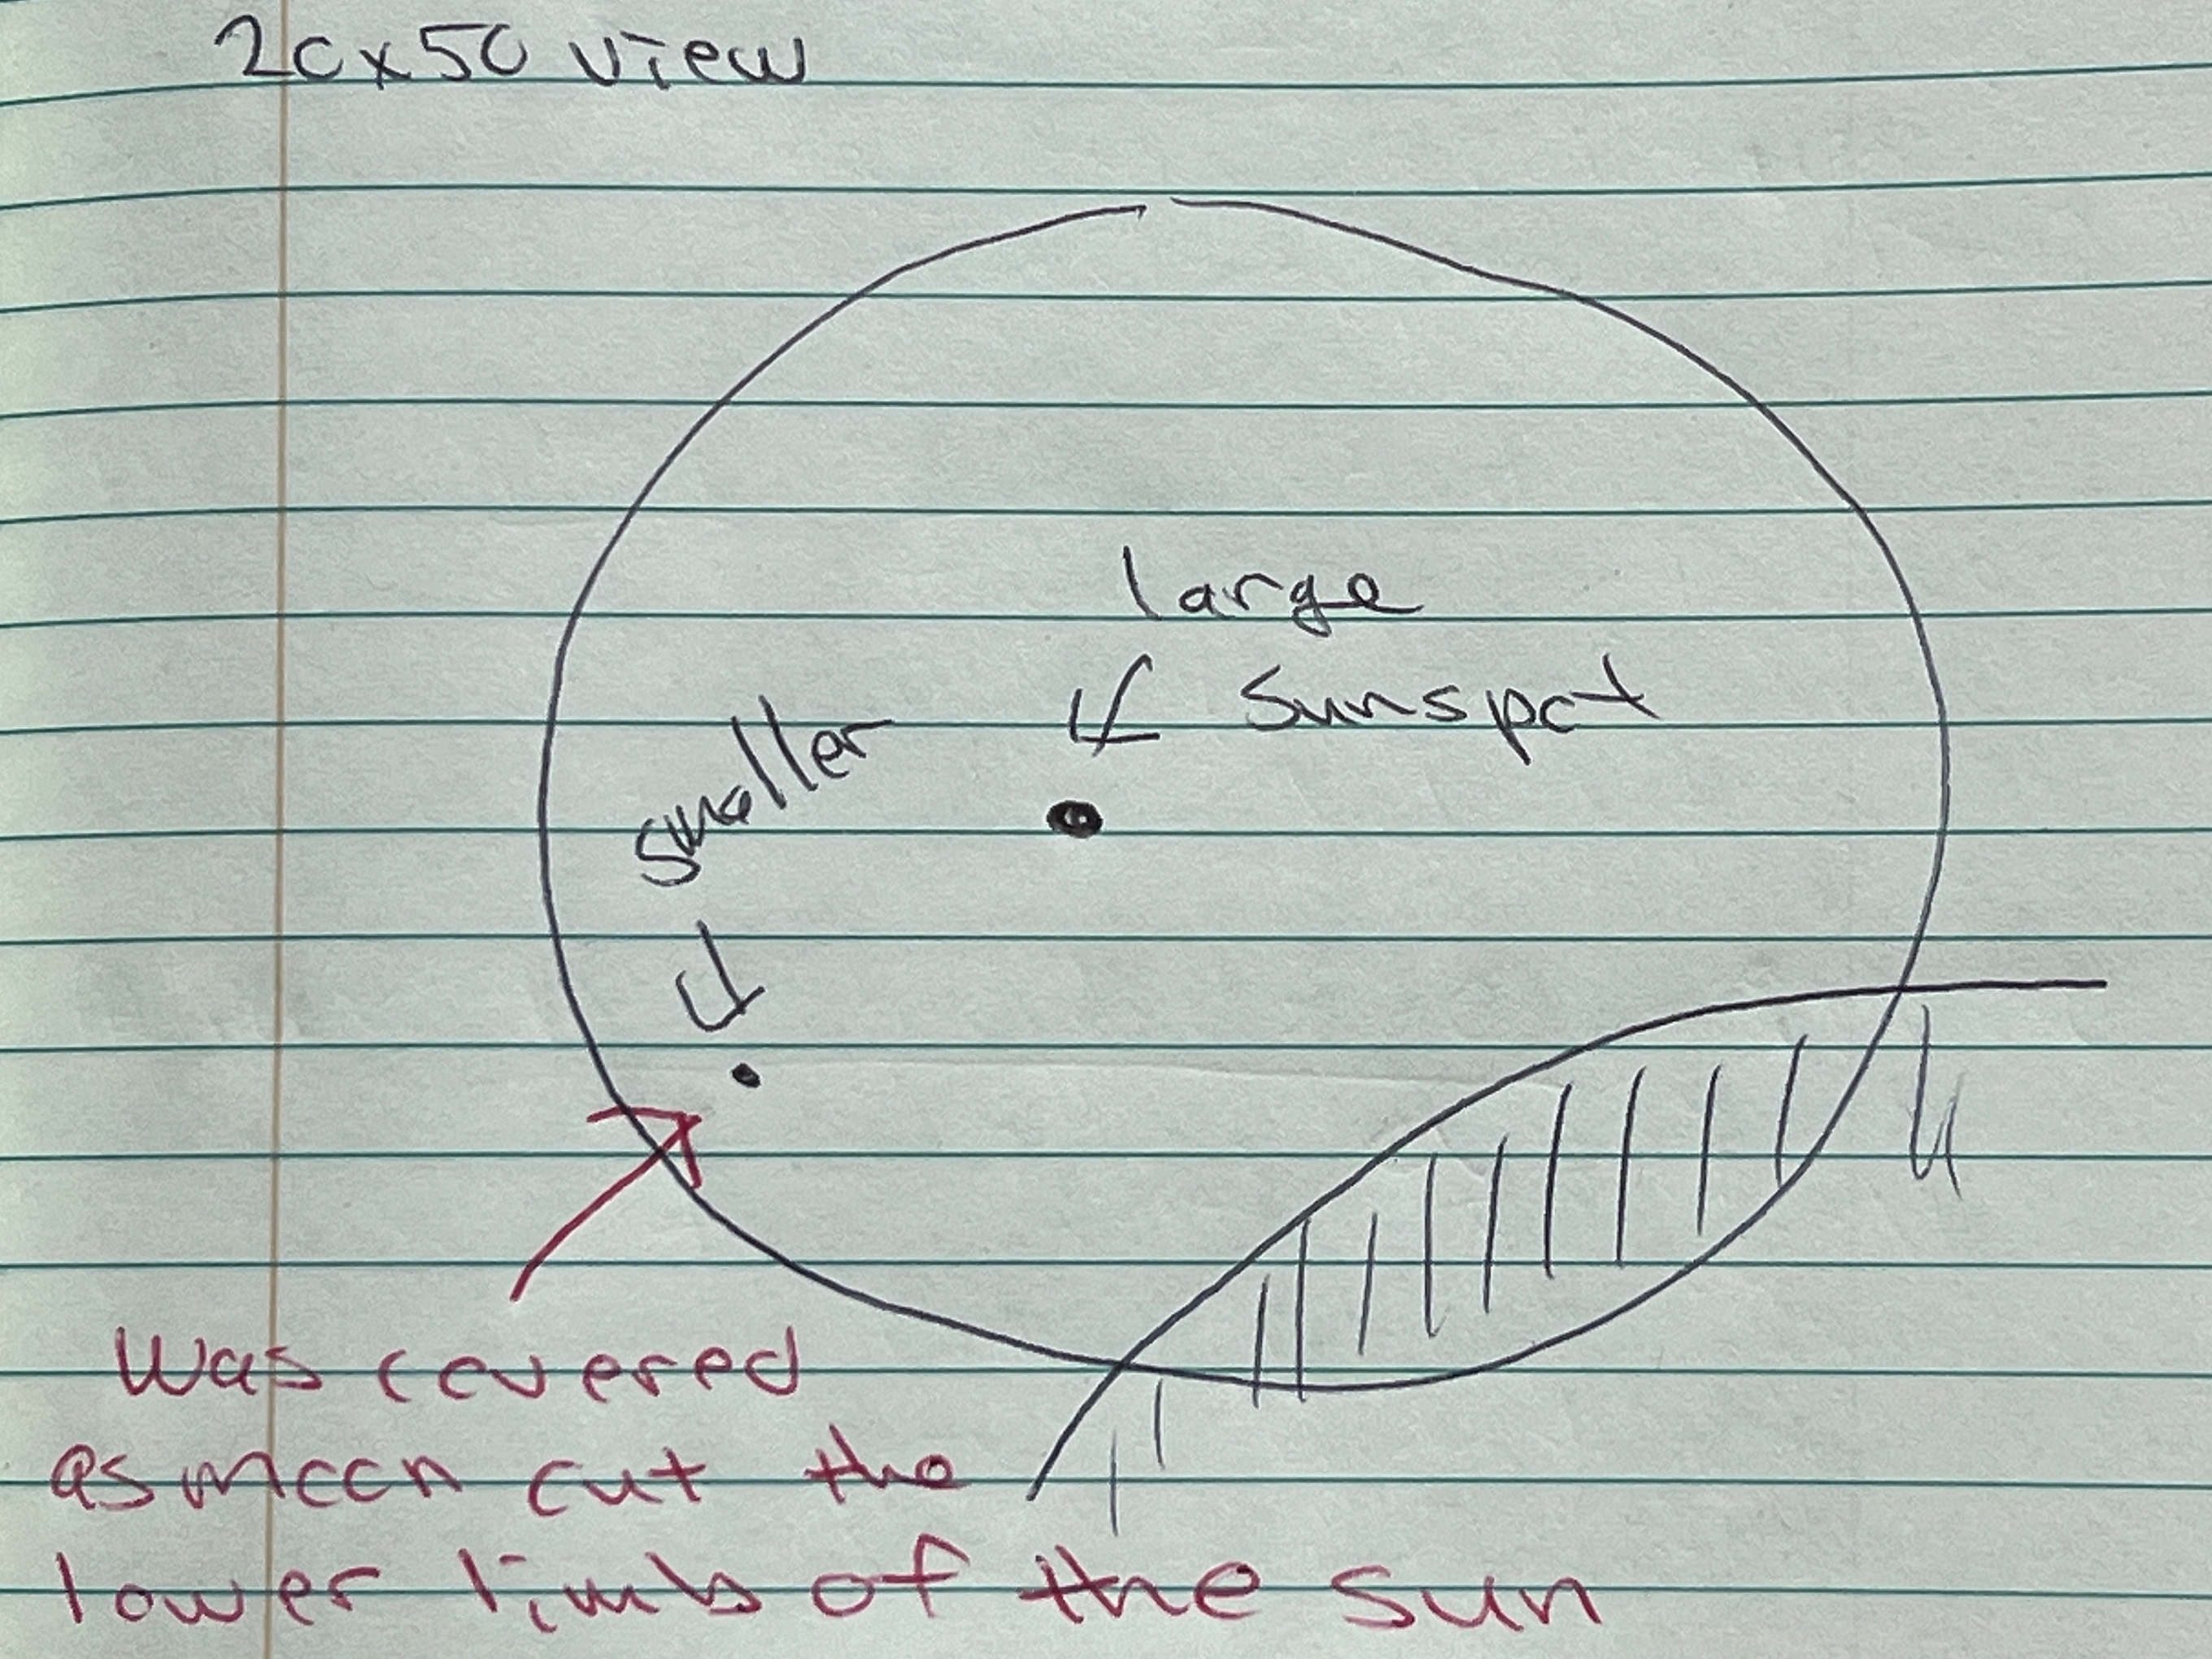
\includegraphics{april_2024_partial_sketch.jpg}
\caption{\emph{Stellar Register} log book sketch of April 8, 2024
partial eclipse from my Idaho backyard}
\end{figure}

While updating my notes, I read my log entry for my first total solar
eclipse. My first total was special, even by total eclipse standards. It
was the first total of the 21\textsuperscript{st} century. I date the
start of the 21\textsuperscript{st} century from this eclipse. Here's my
slightly edited log entry. Pictures from this eclipse trip can be seen
by
\href{https://conceptcontrol.smugmug.com/Trips/Overseas/Zambia-Eclipse-Trip-1}{clicking
here}.

\begin{itemize}
\tightlist
\item
  \emph{Date: June 21, 2001}
\item
  \emph{Site: Zambian schoolyard 89.9 km from Ndeke Hotel}
\item
  \emph{Time: 12:00} \emph{--- 4:00 pm local}
\item
  \emph{GPS Waypoint: ZECLIP}
\item
  \emph{South Latitude: 14.86177} \emph{(degrees)}
\item
  \emph{East Longitude: 27.70558 (degrees)}
\item
  \emph{Elevation: 1158 meters}
\end{itemize}

The eclipse was perfect! I have a feeling I could see the next hundred
eclipses and not top today.

To begin, the weather was perfect. We left the Ndeke Hotel at 8:00 am.
Before leaving, I looked around the sky for clouds, but none could be
seen. The sky remained absolutely clear all day. Better eclipse weather
could not have been catered. The bus ride to the schoolyard
\emph{\href{https://ca.linkedin.com/company/civilized-adventures}{Civilized
Adventures}} had arranged for us was long and dusty. We took the ``great
northern road'' out of Lusaka. About 60 kilometers north of Lusaka, we
turned onto a dusty, unpaved road. For the next 2 ½ hours, the bus
slowly crept the remaining 40 kilometers to the school. All this effort
bought us about twenty seconds of totality. The eclipse was visible from
the Lusaka hotel grounds, and until I saw totality, I wondered if this
ride was worth it.

It was!

We arrived shortly before noon. School kids and their teachers carried
their desks out of the school and set them up under a large tree for our
lunch. We quickly ate lunch and then waited for about one hour. At
1:39:52, the moon touched the sun's disk. I counted down the seconds on
my GPS, then looked up through my pane of welding glass and saw the
moon's disk cut into the sun.

The moon steadily advanced over the sun's disk for the next hour and
twenty minutes. The quality of the light slowly changed. A soft white
evening light filled the soccer field as most of the sun's disk
disappeared. People held up their interlaced fingers and cast crescents
on the ground. Some people poked holes in white cardboard sheets and
projected crescent letters on sheets and t-shirts. ZAMBIA 2001 was a
favorite.

\begin{figure}
\centering
\includegraphics{zambia-2001-41035877.jpg}
\caption{Casting sun crescents during the eclipse onset. Click for a
larger version.}
\end{figure}

As totality approached, Mali and I stood together with others on the
soccer field and watched the sun disappear behind the moon with our
eclipse glasses. At totality, people started yelling. I ripped off my
eclipse glasses and looked up as the last brilliant spike of sunlight
was swallowed up. In its dying flash, a brilliant ring of light with a
huge flare zipped over the sun. People cried, ``The diamond ring.'' It
did look like a diamond ring. Then, instantly, the glare was gone,
leaving a perfect black hole in the sky surrounded by the purest white
corona.

Through binoculars, totality was awesome. The corona was streaming away
from the sun, and brilliant red prominences could be seen on the sun's
edge. Roughly in this pattern:

\begin{figure}
\centering
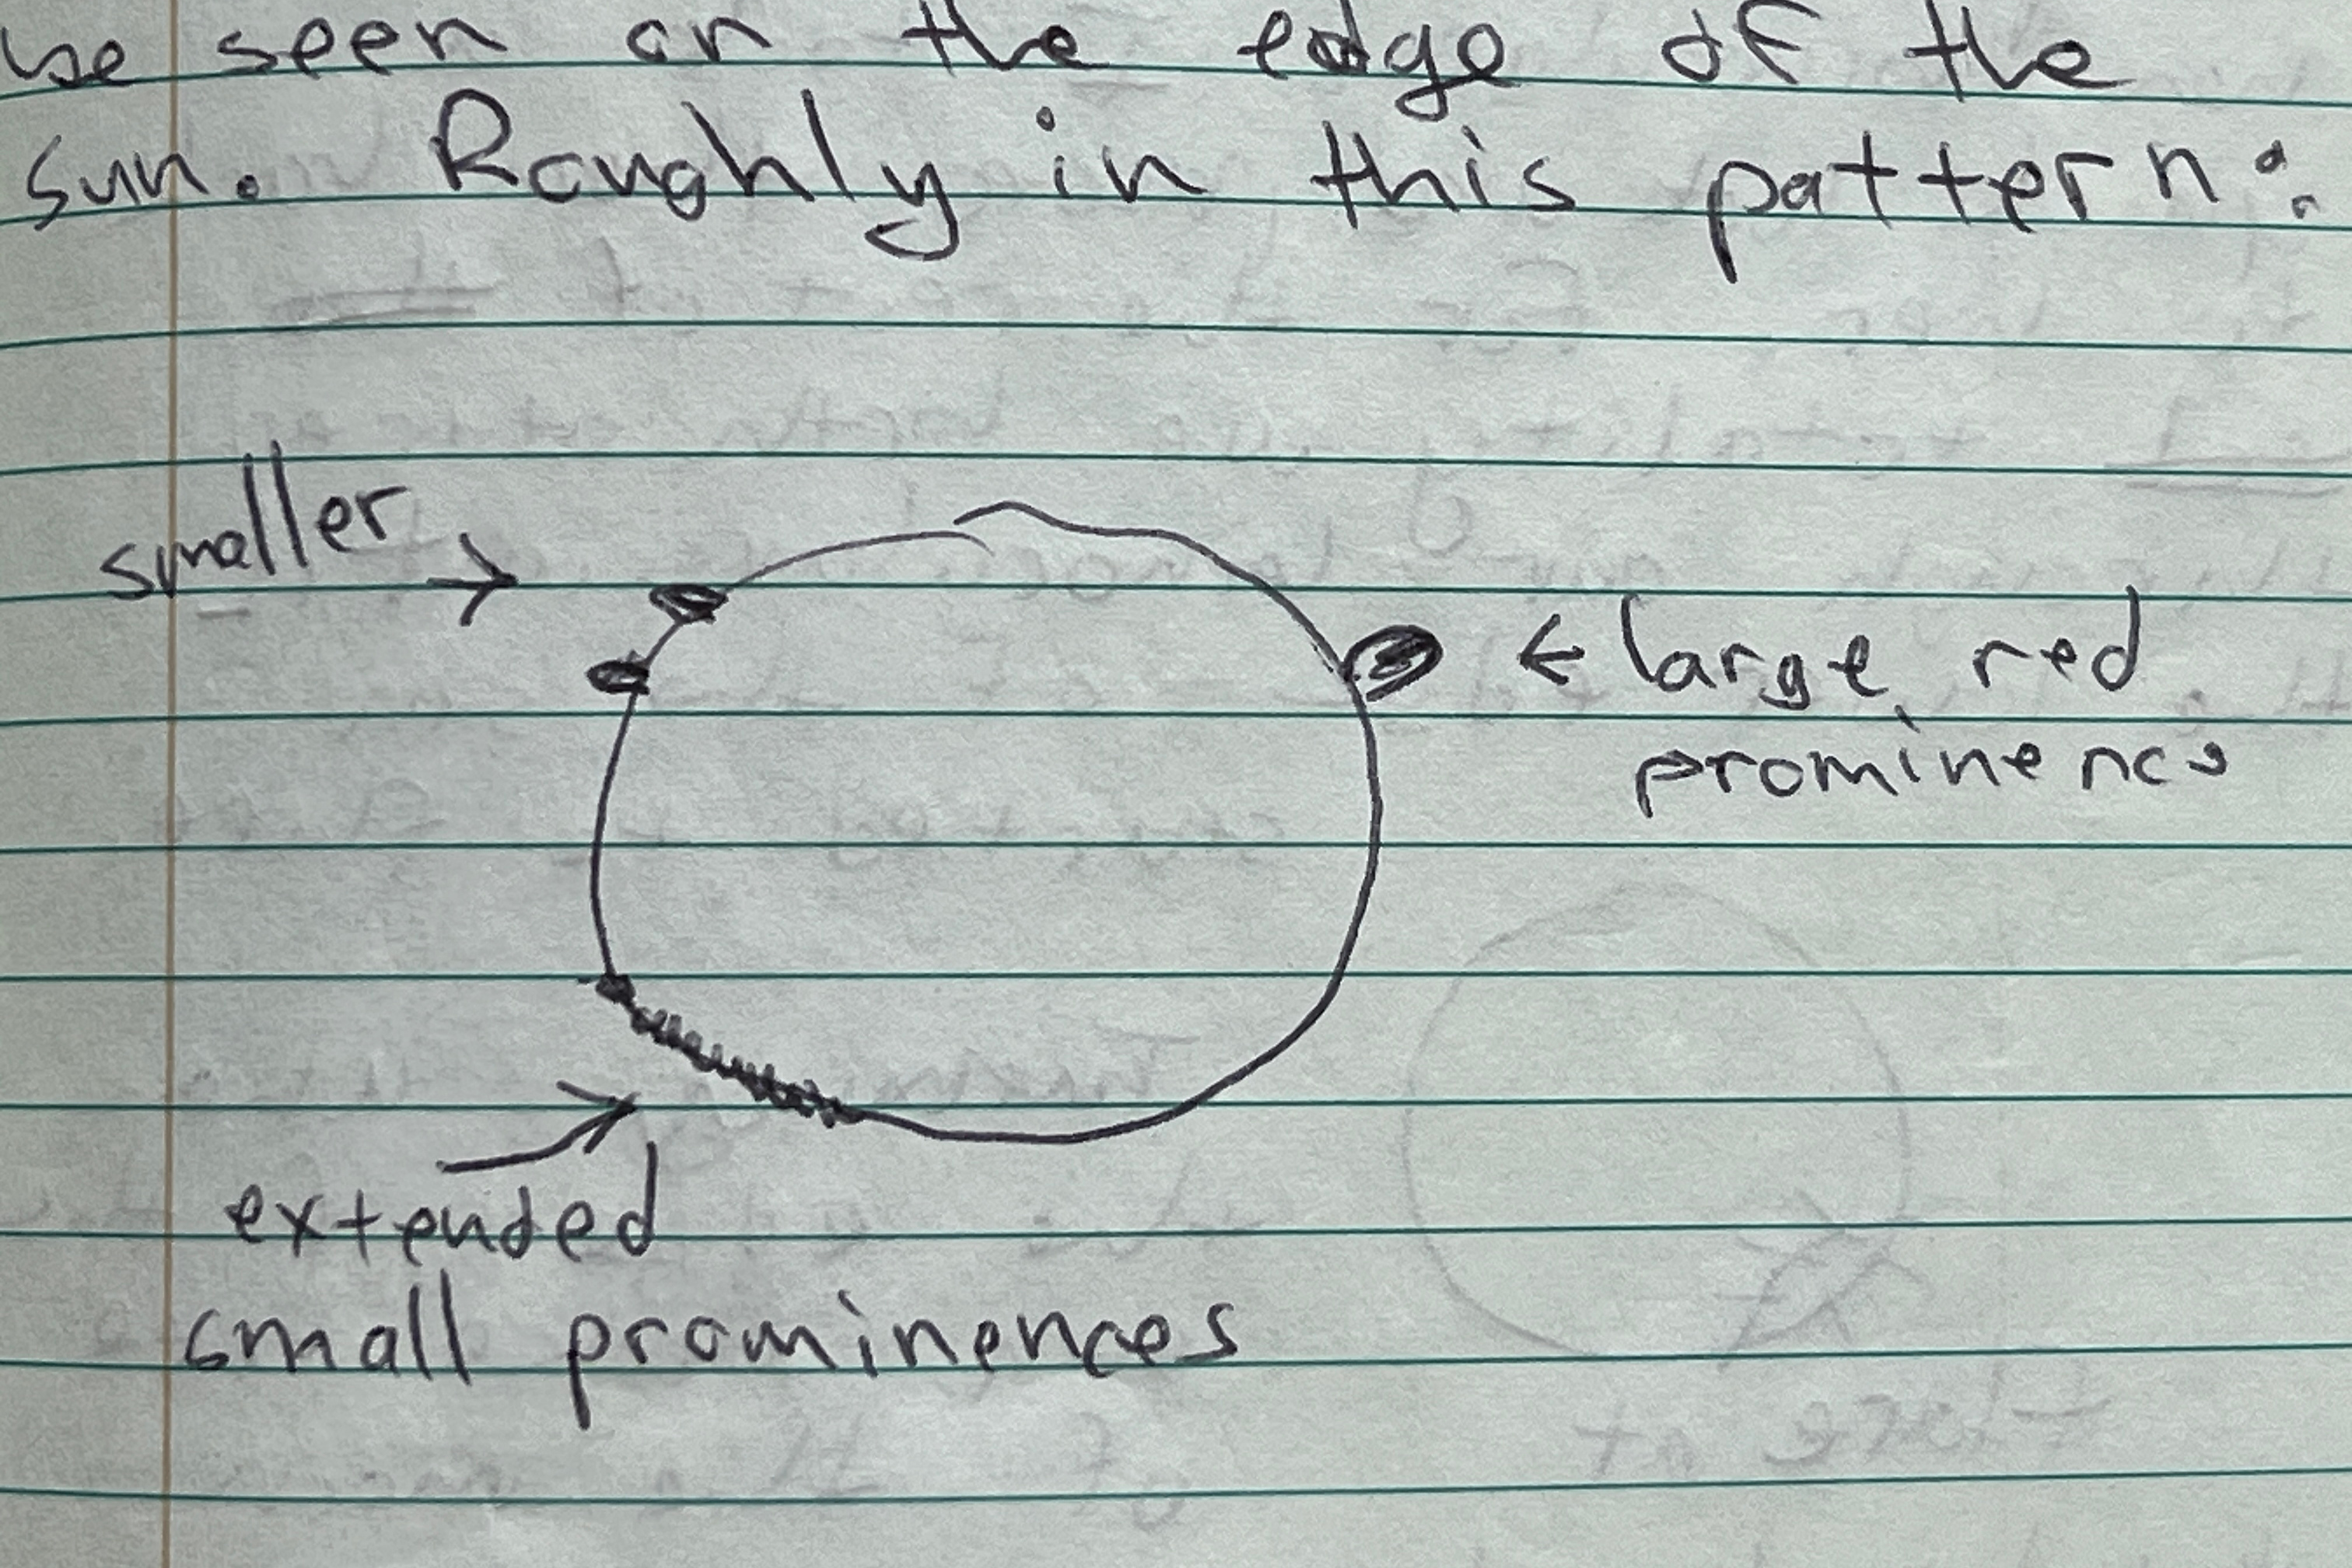
\includegraphics{prominences.jpg}
\caption{My sketch of prominences for the June 21, 2001 eclipse. Click
for photograph.}
\end{figure}

Looking around the sky, which was as dark as twilight, I could see three
objects: Jupiter, Sirius, and Saturn to the east. There was a sunset
glow low on all horizons.

Dropping my binoculars, I stared at the eclipse. The moon was a perfect
black dot backlit by pure corona. On the ground, we saw ``shadow band''
ripples of light. Mali started yelling about the prominences and handed
me her binoculars. I took a quick look and passed them back to her. For
the rest of totality, we both stared through our binoculars until the
lower edge of the sun started to flare.

\begin{figure}
\centering
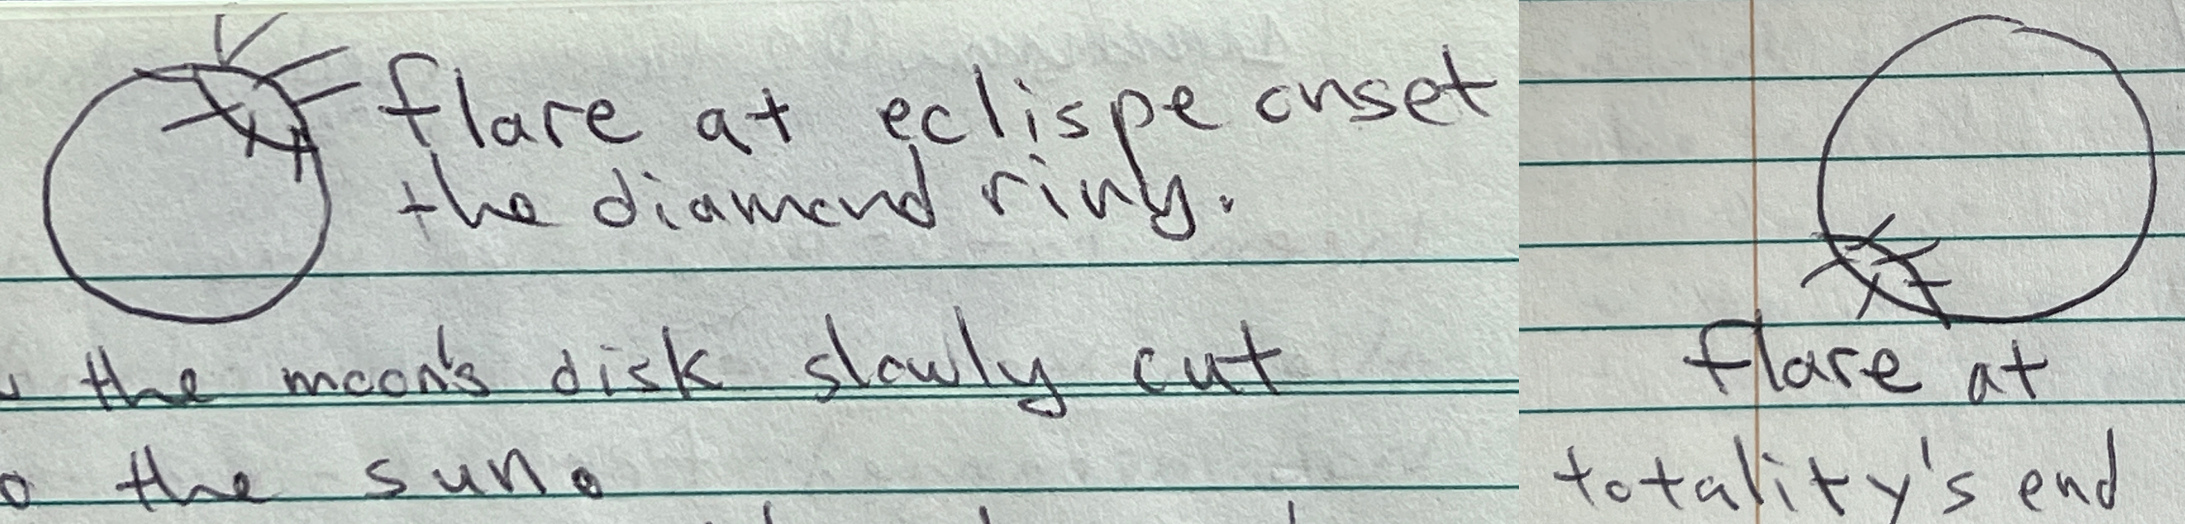
\includegraphics{eclipse_begin_end_flares.jpg}
\caption{My rough sketches of the flares at the start and end of the
June 21, 2001 eclipse.}
\end{figure}

When the sun's edge broke free of the moon, I turned away and looked at
the crowd as sunlight levels increased. It is amazing how bright the
smallest sliver of the sun's disk is. When just a dot of the sun
returned, it was instantly daylight again, a weird blue dim daylight but
still daylight. I couldn't believe that over three minutes had passed.
They were the shortest three minutes of my life.

Two words about total solar eclipses: \textbf{HIGHLY RECOMMENDED!}

\emph{Also, 20 on a scale of 10! Three thumbs up! Really better than\\
sex!}

\begin{figure}
\centering
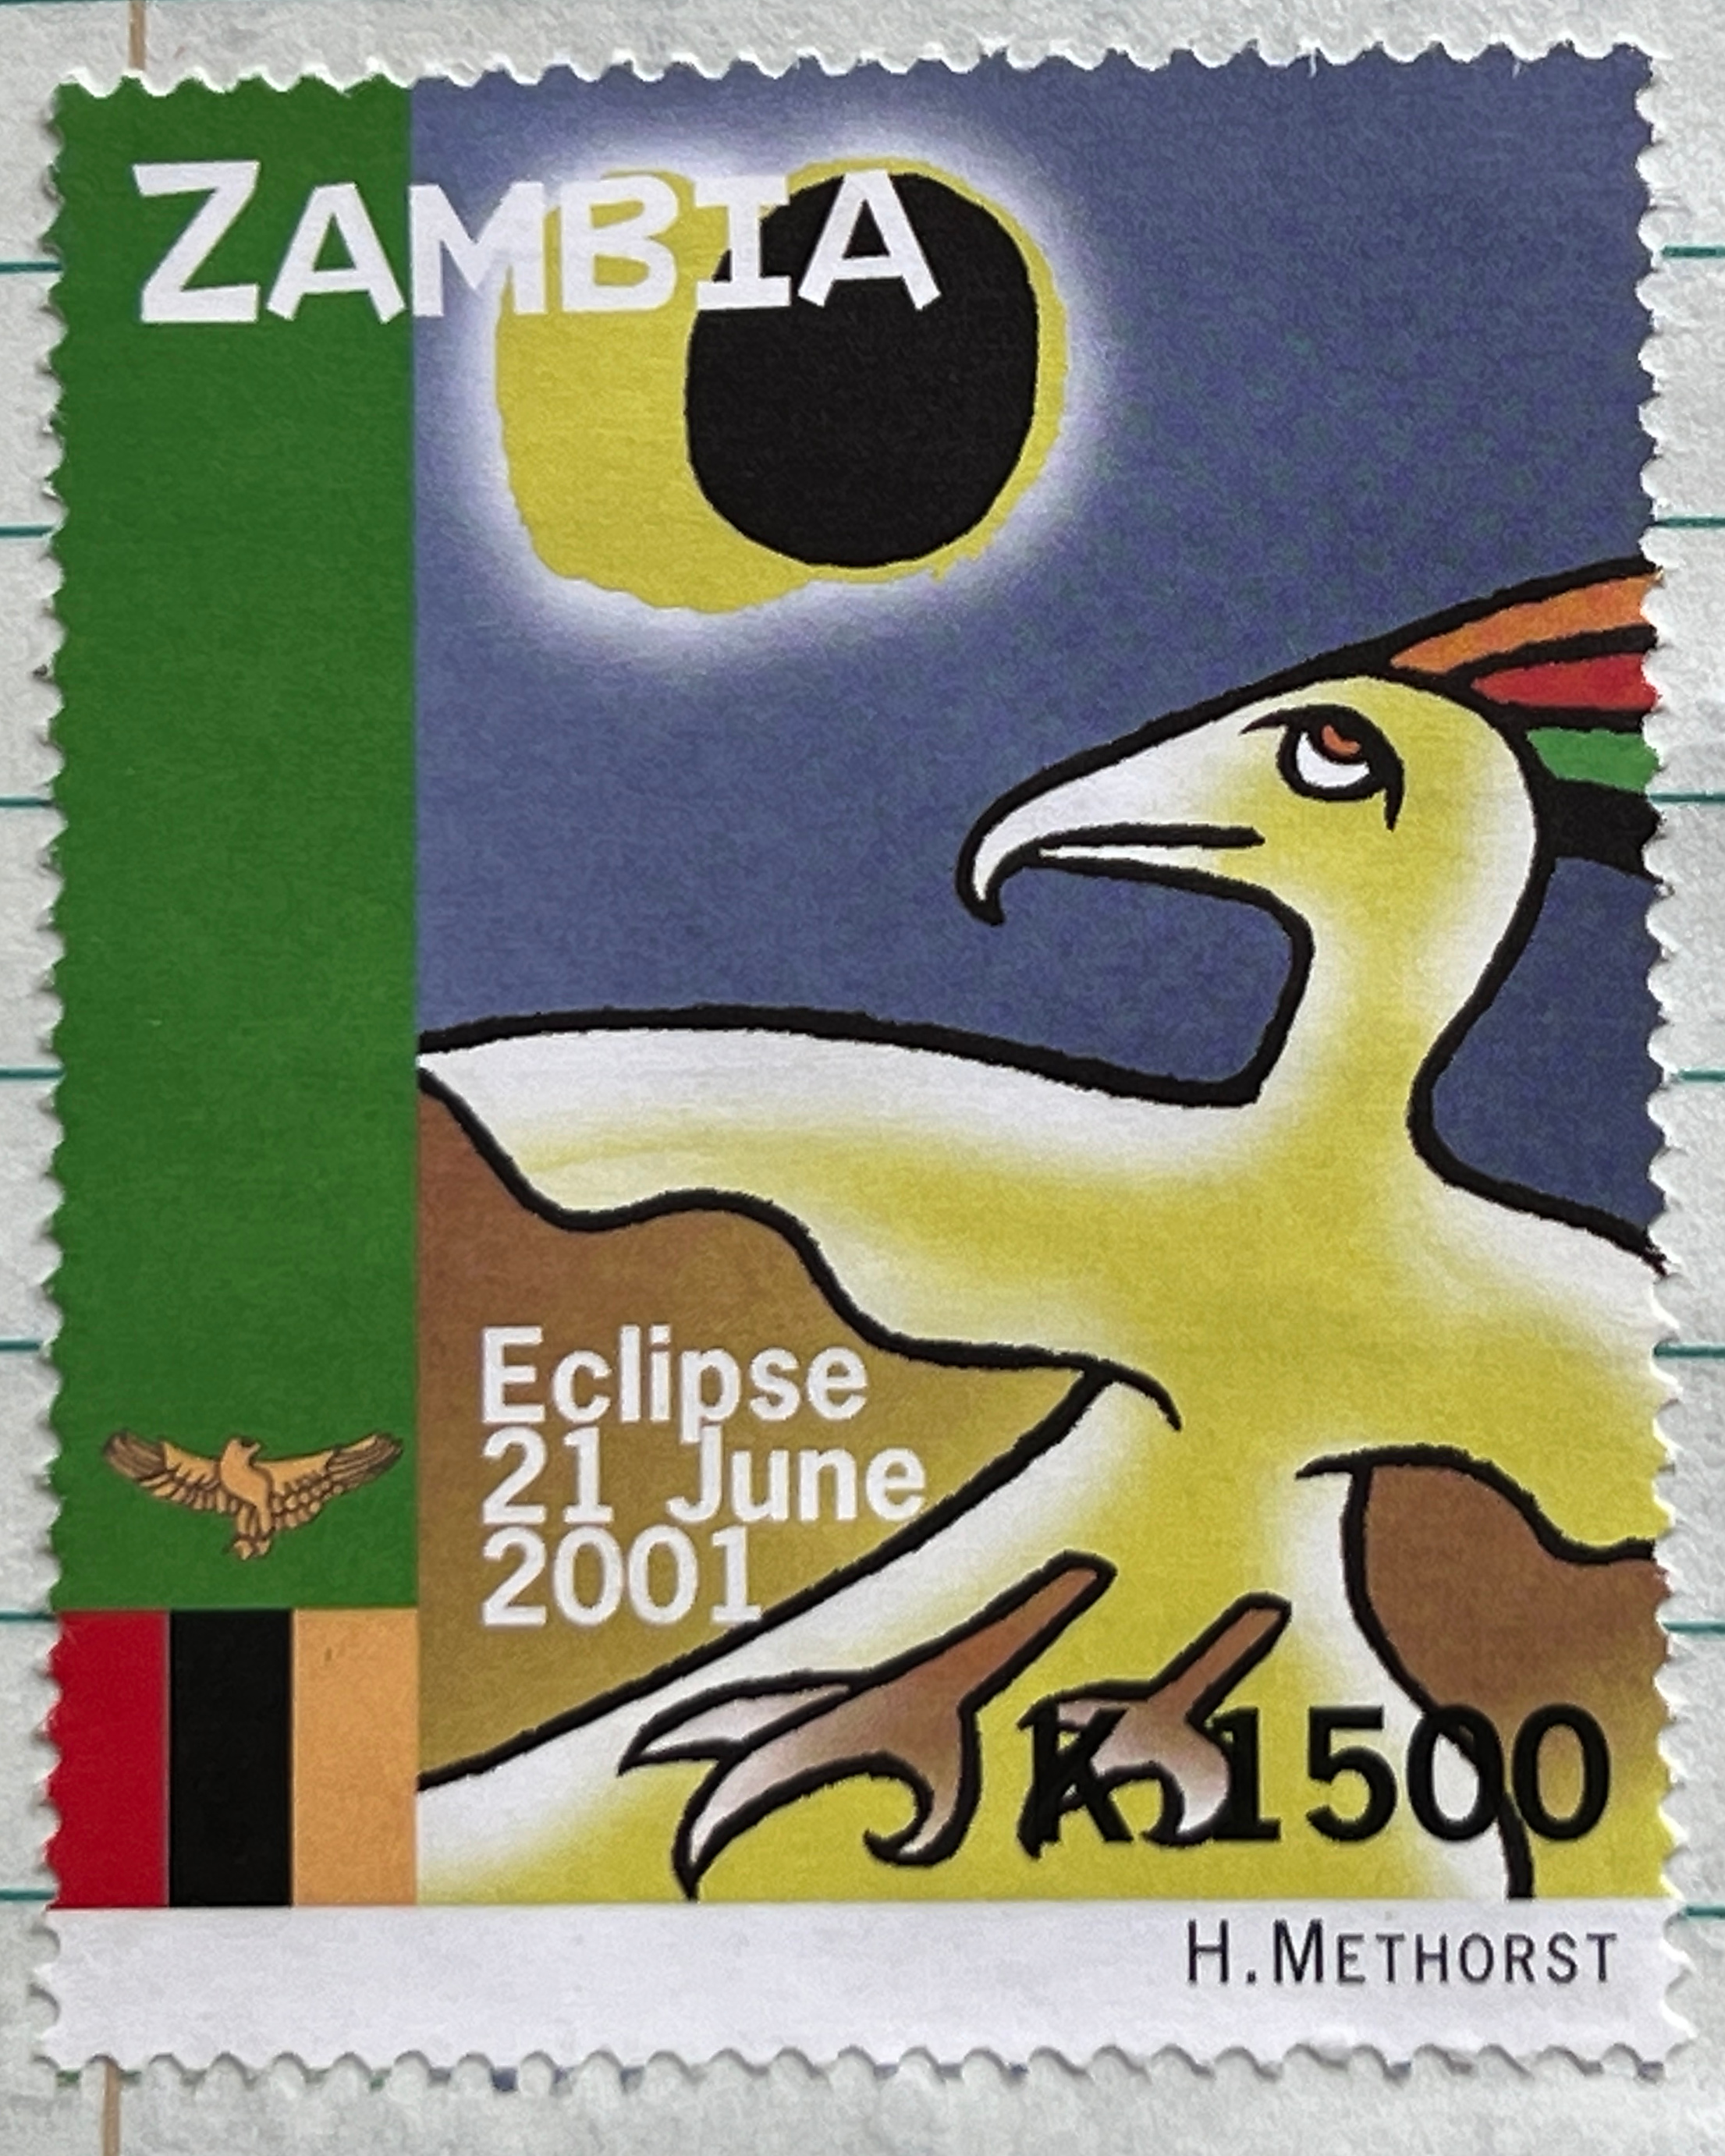
\includegraphics{2001_eclipse_stamp.jpg}
\caption{Stamp celebrating the June 21, 2001 eclipse. The first total
solar eclipse of the 21st century. Click for image gallery.}
\end{figure}

%\captionsetup[floatingfigure]{labelformat=empty}
%\begin{figure}[htbp]
%\begin{floatingfigure}[l]{0.25\textwidth}
%\centering
%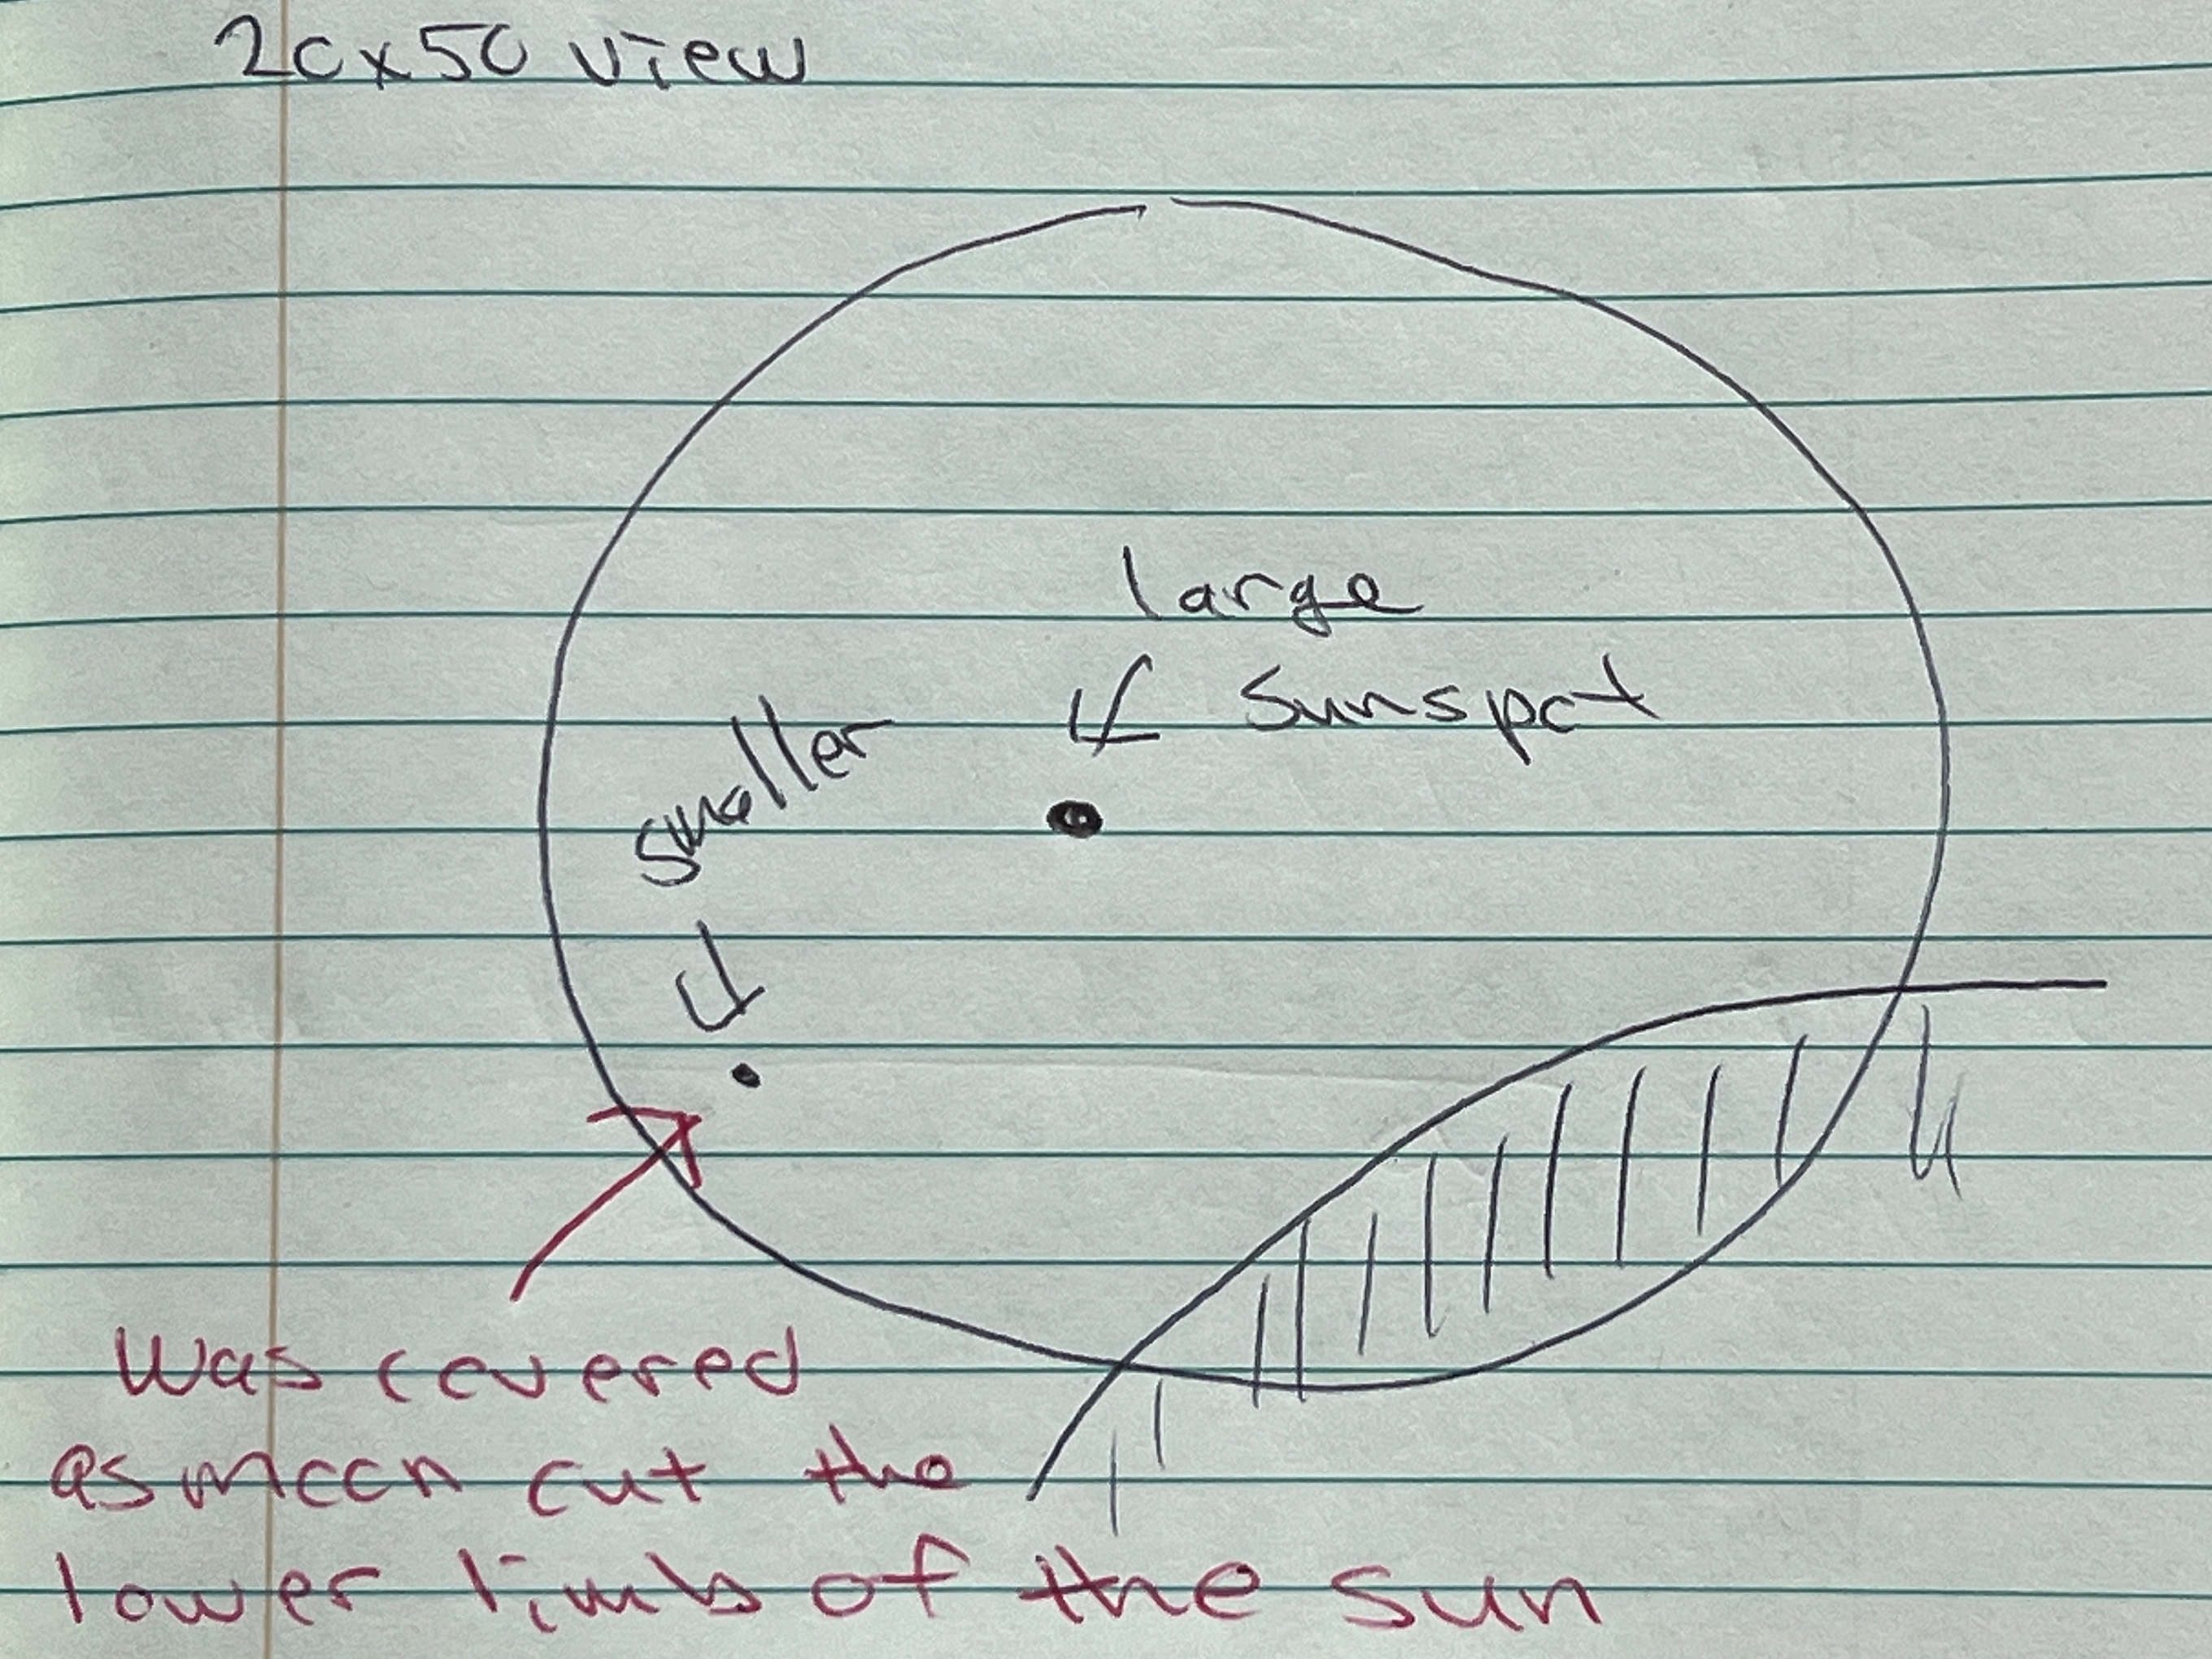
\includegraphics[width=0.23\textwidth]{april_2024_partial_sketch.jpg}
%\caption{~~~IMCAPTION~~~}
%\label{fig:8074X0}
%\end{floatingfigure}
%\end{figure}

%\captionsetup[floatingfigure]{labelformat=empty}
%\begin{figure}[htbp]
%\begin{floatingfigure}[l]{0.25\textwidth}
%\centering
%\includegraphics[width=0.23\textwidth]{zambia-2001-41035877.jpg}
%\caption{~~~IMCAPTION~~~}
%\label{fig:8074X1}
%\end{floatingfigure}
%\end{figure}

%\captionsetup[floatingfigure]{labelformat=empty}
%\begin{figure}[htbp]
%\begin{floatingfigure}[l]{0.25\textwidth}
%\centering
%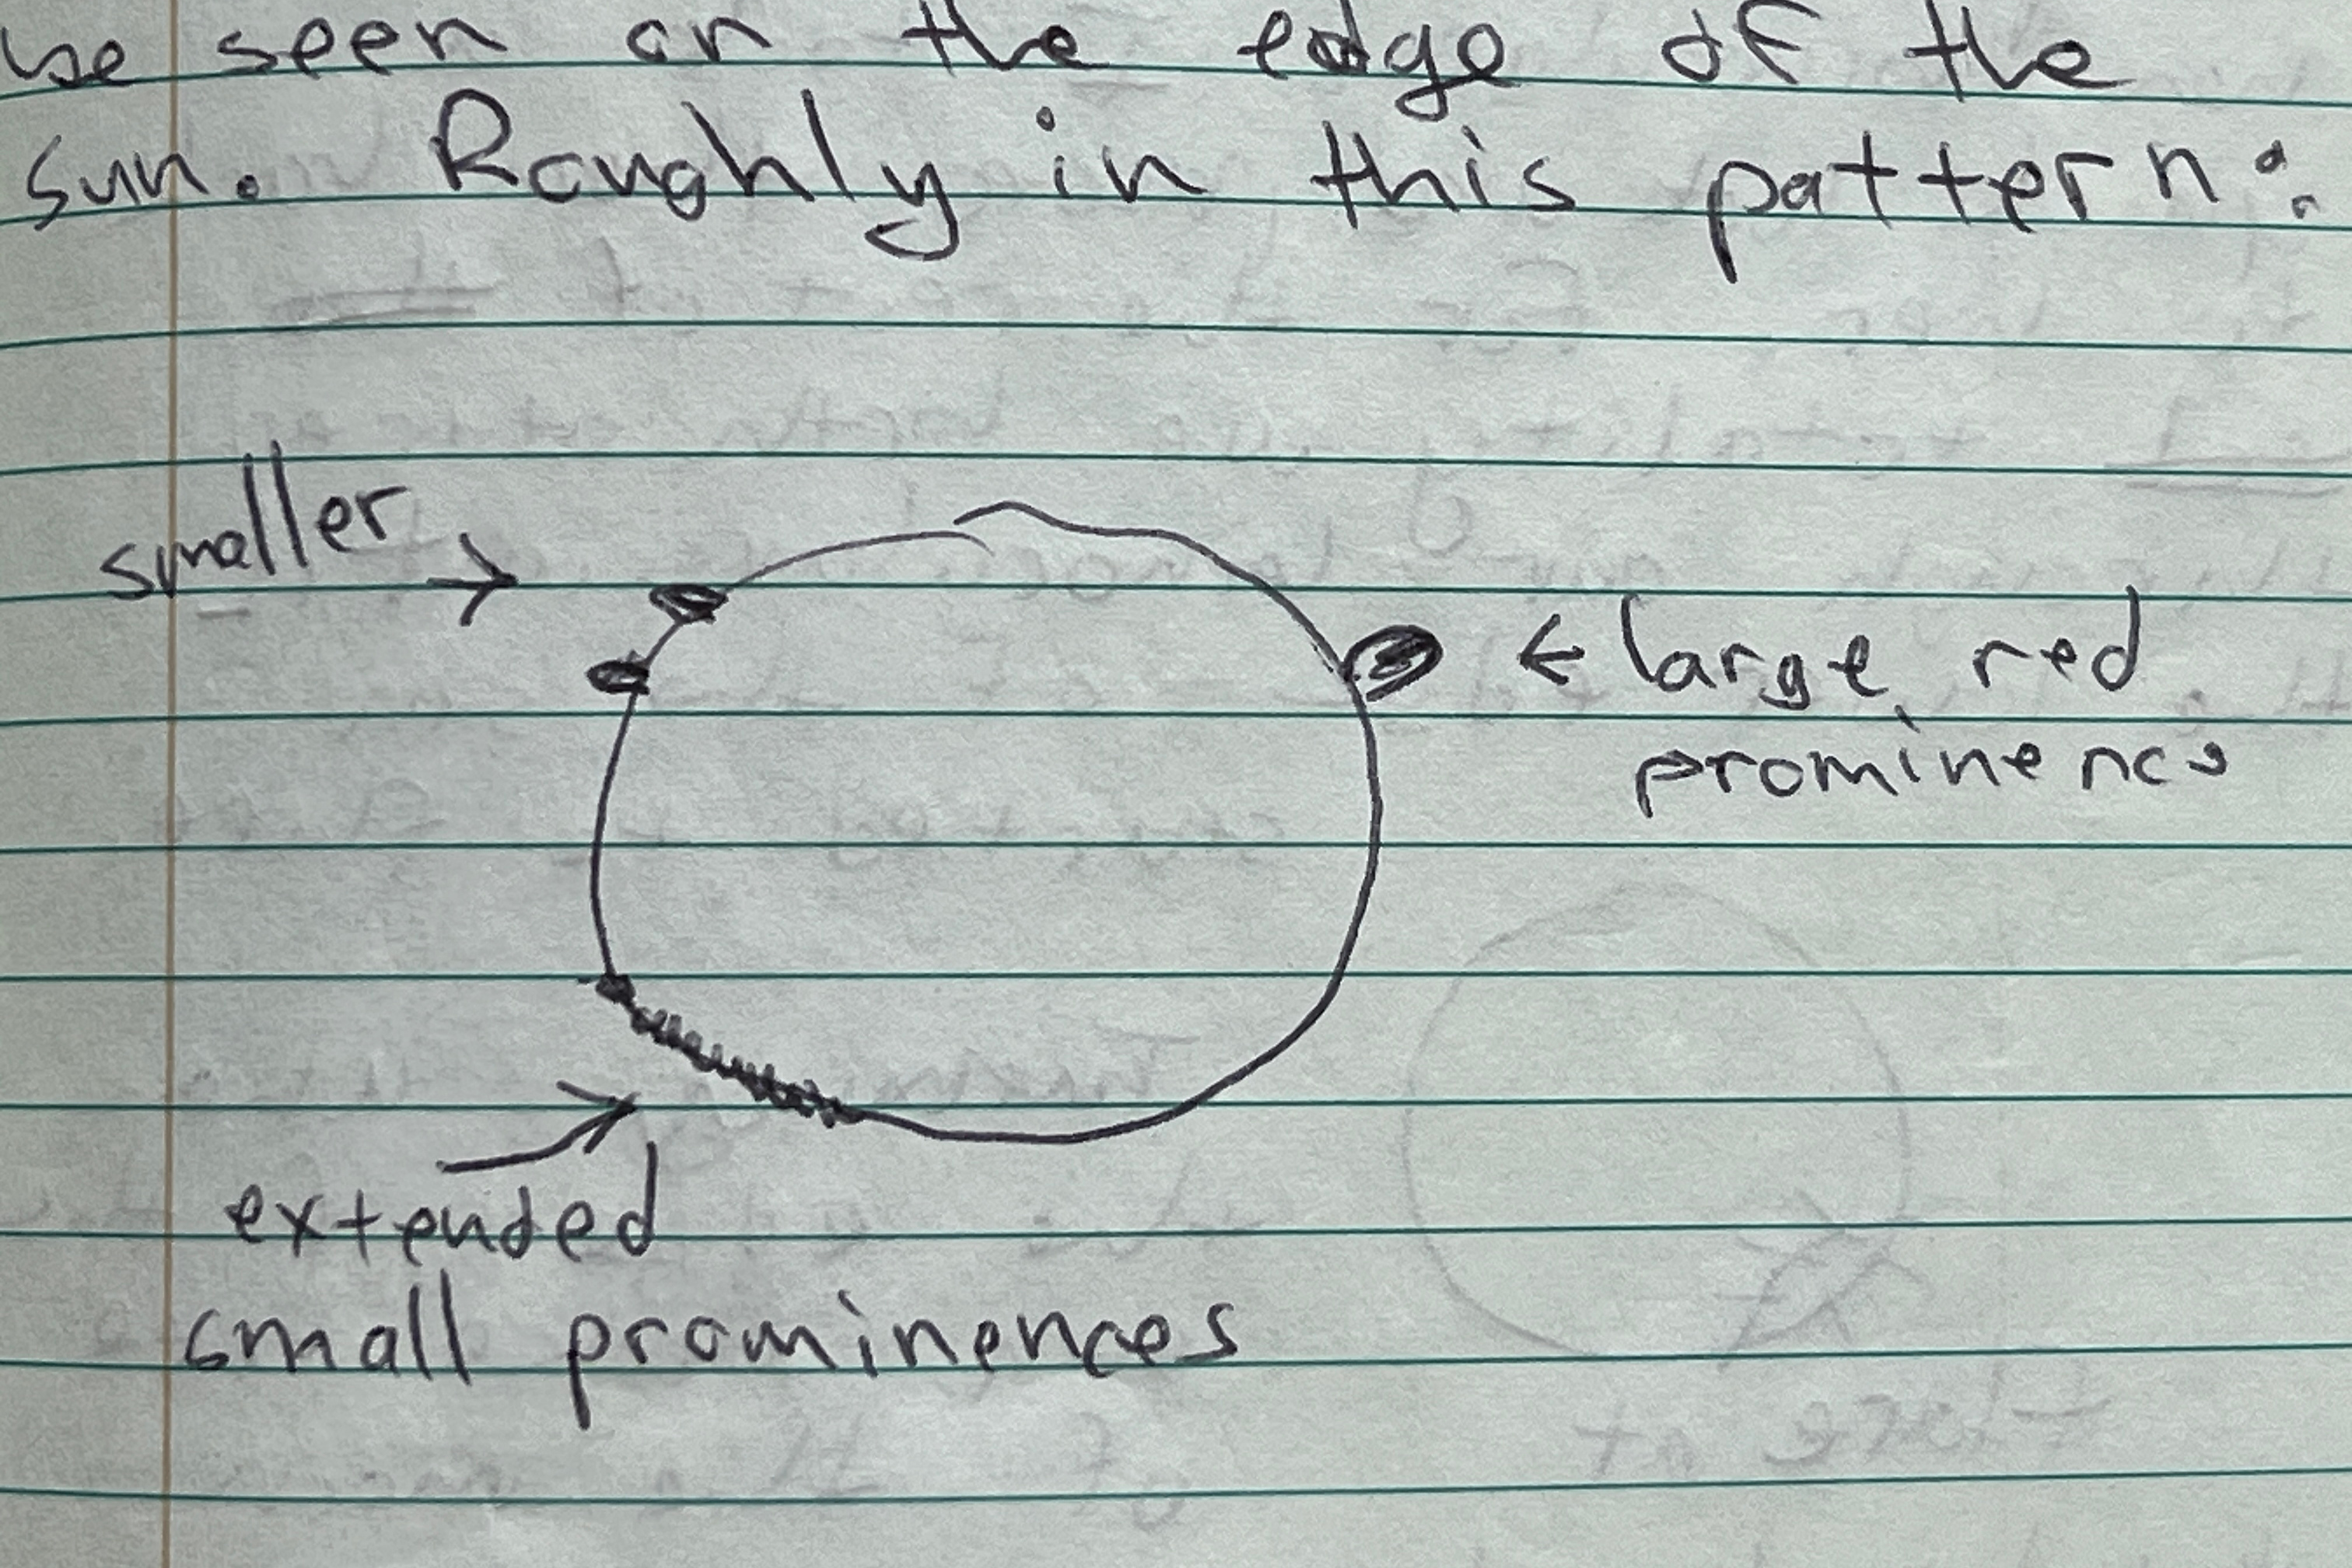
\includegraphics[width=0.23\textwidth]{prominences.jpg}
%\caption{~~~IMCAPTION~~~}
%\label{fig:8074X2}
%\end{floatingfigure}
%\end{figure}

%\captionsetup[floatingfigure]{labelformat=empty}
%\begin{figure}[htbp]
%\begin{floatingfigure}[l]{0.25\textwidth}
%\centering
%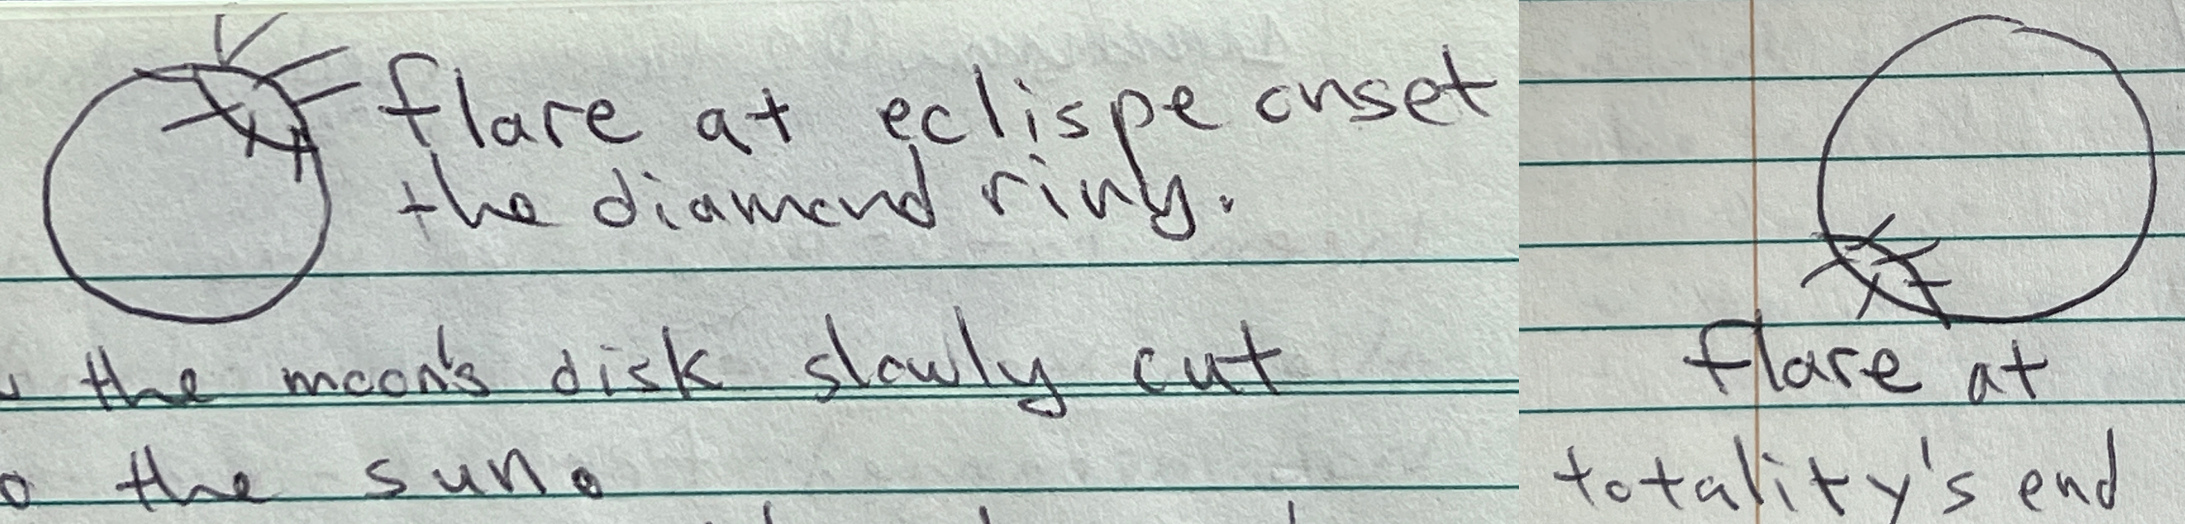
\includegraphics[width=0.23\textwidth]{eclipse_begin_end_flares.jpg}
%\caption{~~~IMCAPTION~~~}
%\label{fig:8074X3}
%\end{floatingfigure}
%\end{figure}

%\captionsetup[floatingfigure]{labelformat=empty}
%\begin{figure}[htbp]
%\begin{floatingfigure}[l]{0.25\textwidth}
%\centering
%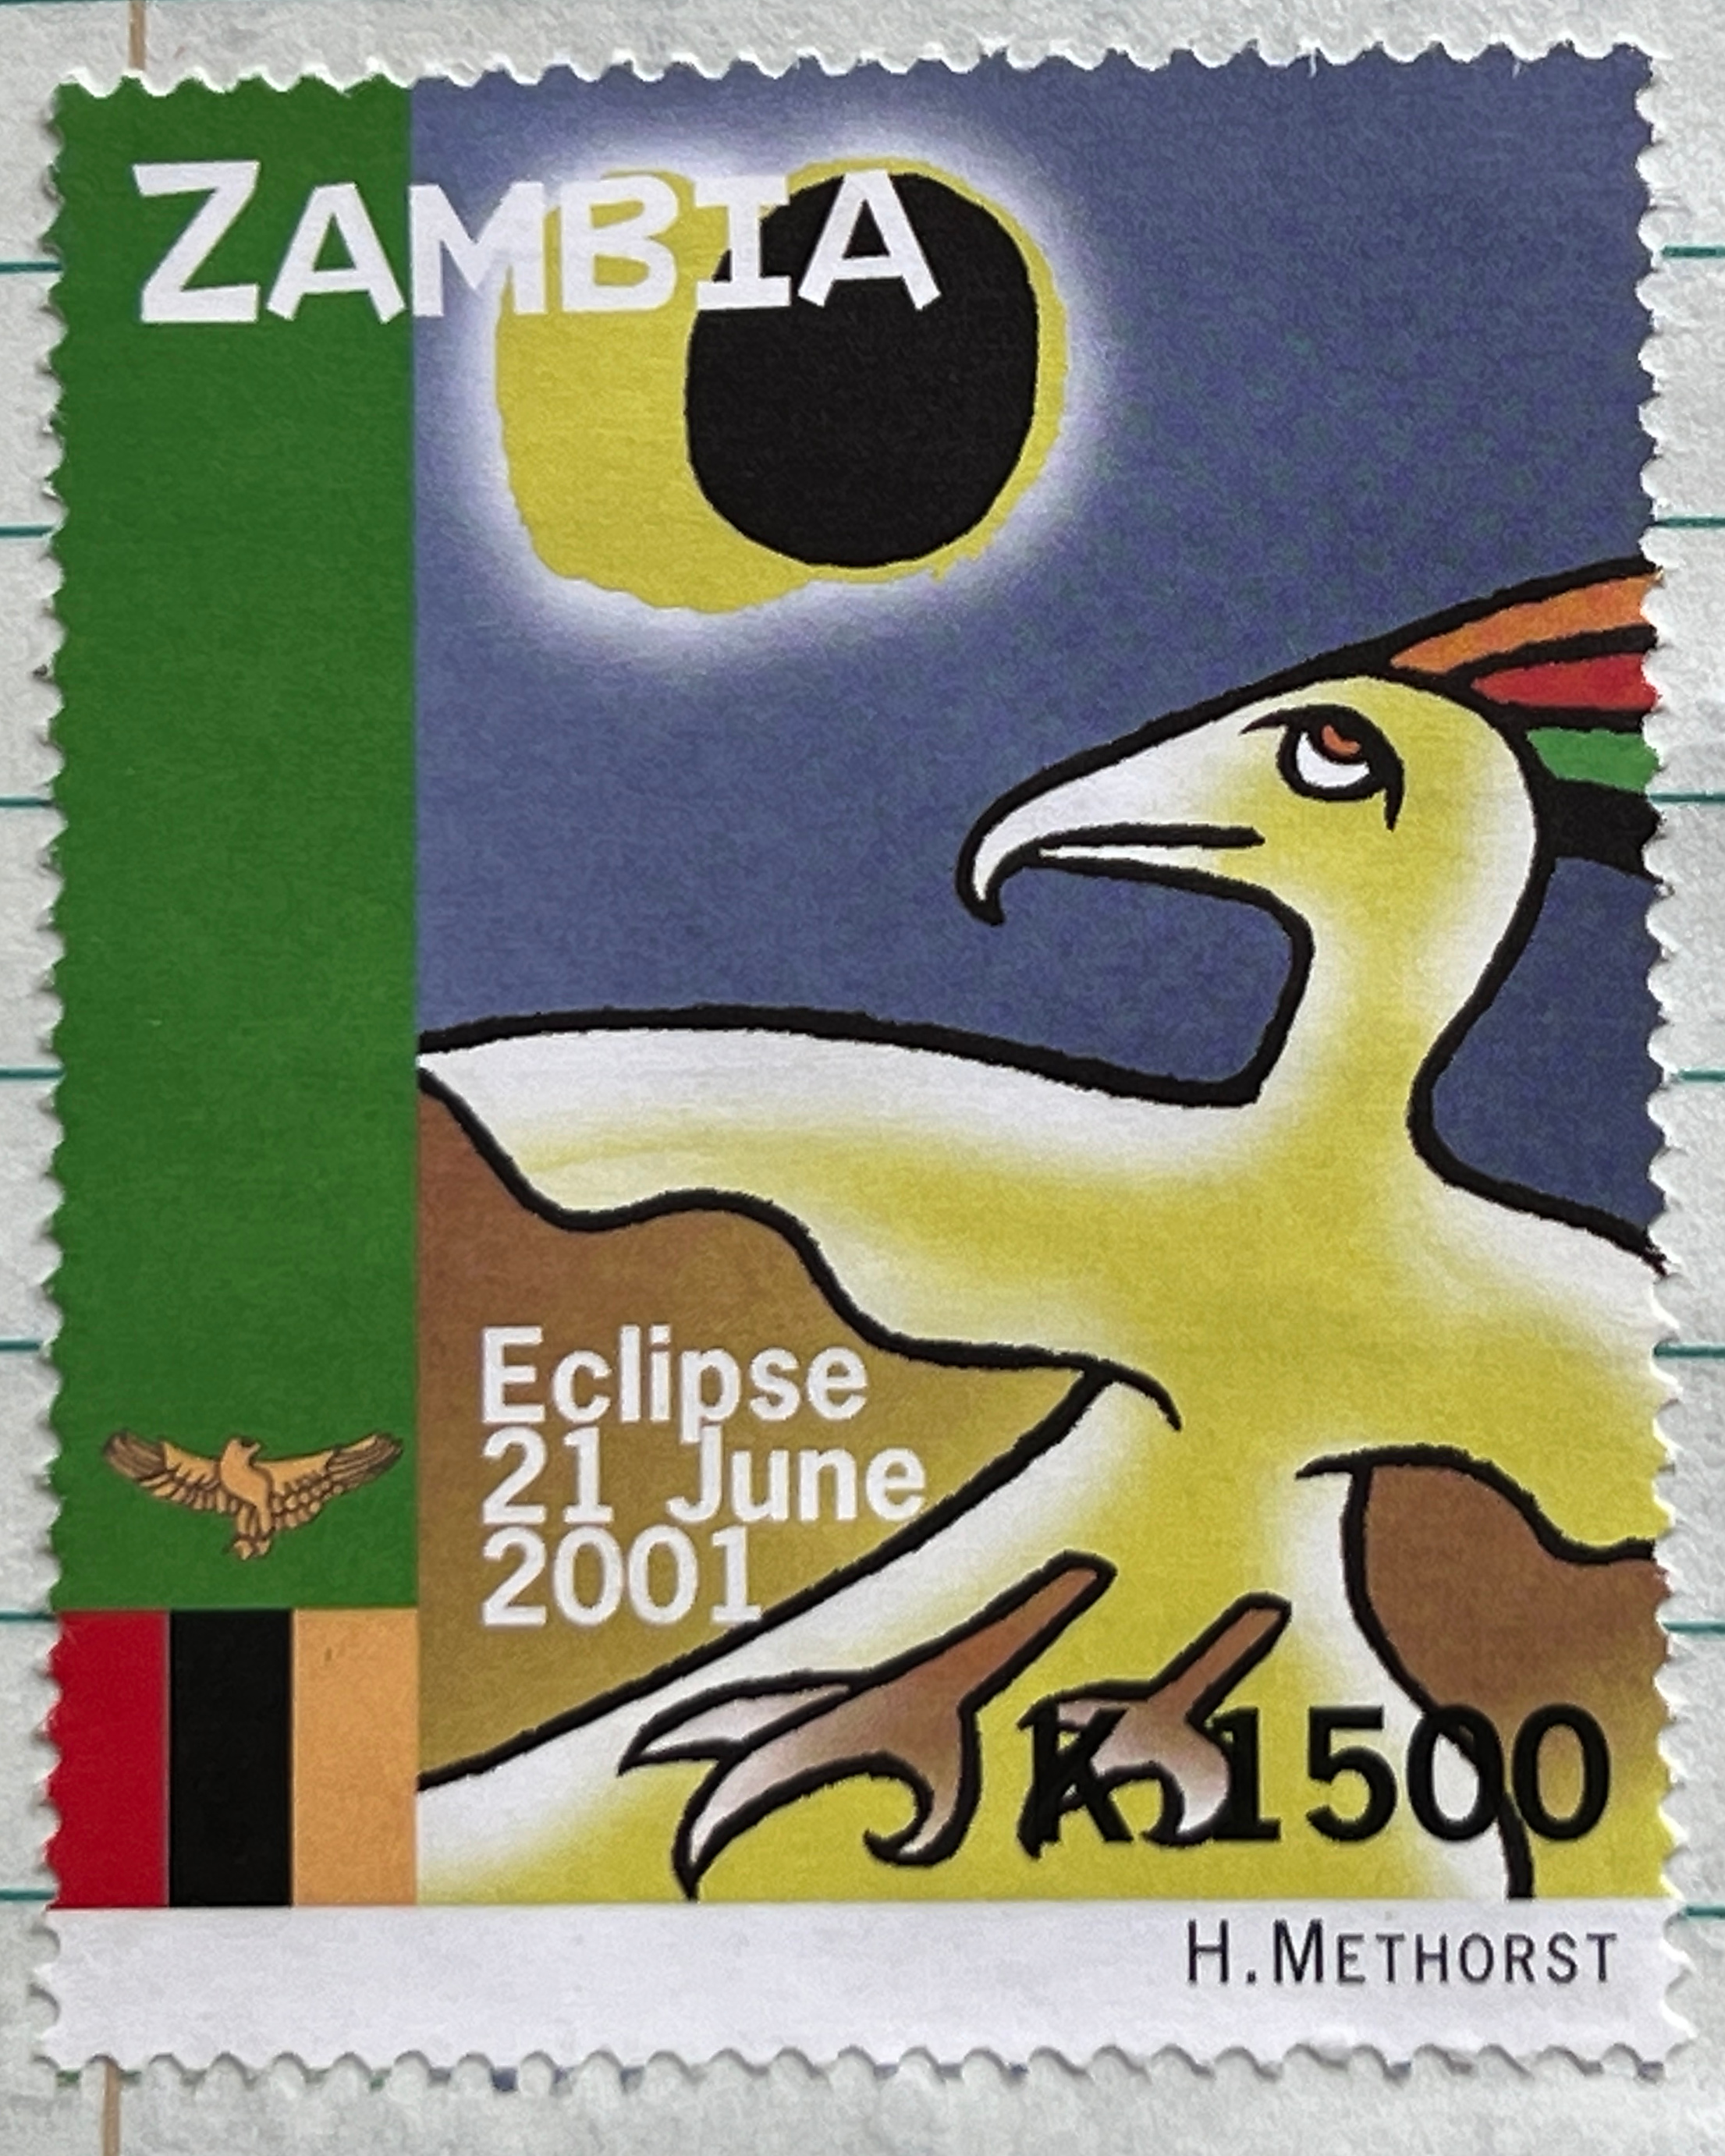
\includegraphics[width=0.23\textwidth]{2001_eclipse_stamp.jpg}
%\caption{~~~IMCAPTION~~~}
%\label{fig:8074X4}
%\end{floatingfigure}
%\end{figure}



%\end{document}
 
% standard floating figure
% \captionsetup[figure]{labelformat=empty}
% \begin{figure}[htbp]
% \centering
% \href{}{\includegraphics[width=0.50\textwidth]{}}
% \caption{}
% \label{fig:????x0}
% \end{figure}
 
% captions beside figure
% \captionsetup[figure]{labelformat=empty}
% \begin{SCfigure}
% \centering
% \href{}{\includegraphics[width=0.40\textwidth]{}}
% \caption{}
% \label{fig:????x0}
% \end{SCfigure}
 
% wrapped figure - outer size > inner size
% \captionsetup[floatingfigure]{labelformat=empty}
% \begin{floatingfigure}[l]{0.23\textwidth}
% \centering
% \href{}{\includegraphics[width=0.22\textwidth]{}}
% \caption{}
% \label{fig:????x0}
% \end{floatingfigure}
